% DATA404 Multimodal Machine Learning -- final project deck.
%
% Build:  latexmk -pdf slides.tex        (from this directory)
%
% Written to be read by someone outside the project. Every abbreviation is
% expanded, every number carries its interpretation, and no slide depends on
% an internal run or decision identifier to make sense. Run identifiers appear
% only as small provenance tags, explained once on the "How to read" slide.
%
% Every number here comes from a registered run under ../results/ and is
% checked against those files by slides/check_slide_numbers.py.
\documentclass[aspectratio=169,10pt]{beamer}

\usetheme[workplace=vsu]{MU}

\usepackage[T1]{fontenc}
\usepackage[utf8]{inputenc}
\usepackage{booktabs}
\usepackage{array}

% A small grey provenance tag. Never the only thing identifying a result.
\newcommand{\runtag}[1]{{\scriptsize\color{mubeamer@gray7}[#1]}}
\newcommand{\sidenote}[1]{{\scriptsize\color{mubeamer@gray7}\sloppy\par#1\par}}
\newcommand{\reads}[1]{\textbf{How to read this:} #1}

\title[Can eye tracking and heart signals match EEG?]%
      {Can eye tracking and heart signals match brain recording?}
\subtitle{Predicting how much a learner remembers from an educational video,
  for learners the model has never seen}
\author[Bhatt \& Tanmayee]{Priyanka Bhatt (2023UG000127) \and Tanmayee K M (2023UG000134)}
\institute{DATA404 Multimodal Machine Learning \\ Vidyashilp University
  \quad$\cdot$\quad Dr.\ Minati Rath}
\date{}

\begin{document}

\begin{frame}[plain]
  \titlepage
\end{frame}

% ---------------------------------------------------------------- question
\begin{frame}{The question we set out to answer}
  \begin{block}{Motivation}
    Research in educational neuroscience predicts how much a student learns
    from \textbf{EEG} --- electroencephalography, which records electrical
    brain activity through electrodes on the scalp. EEG is expensive,
    uncomfortable, and impractical in a classroom.
  \end{block}

  \vspace{0.4em}
  \begin{block}{Our question}
    Can \textbf{cheaper, less intrusive sensors} --- an eye tracker, and
    \textbf{ECG} (electrocardiography, a heart-activity recording) --- predict
    learning as well as EEG does? And does combining several sensors predict
    better than the best single one?
  \end{block}

  \vspace{0.4em}
  \begin{itemize}\small
    \item \textbf{What we predict:} the proportion of memory questions a
      learner answers correctly after watching a video, standardised within
      each video so that videos of different difficulty are comparable.
    \item \textbf{Who we predict for:} learners the model has \emph{never seen}
      --- much harder than predicting a new video for a known learner.
    \item \textbf{What we predict from:} that learner's own signals only, never
      their similarity to the group.
  \end{itemize}
\end{frame}

% ---------------------------------------------------------------- glossary
\begin{frame}{How to read these slides}
  \small
  \begin{columns}[T]
    \begin{column}{0.49\textwidth}
      \textbf{Terms used throughout}
      \begin{itemize}\small
        \item \textbf{EEG} --- electroencephalography, brain electrical
          activity from scalp electrodes.
        \item \textbf{ECG} --- electrocardiography, heart electrical activity.
        \item \textbf{Saccade} --- a rapid jump of the eyes between points.
          \textbf{Fixation} --- a pause between saccades.
        \item \textbf{Attentive / distracted} --- the two viewing conditions
          in the dataset. Learners watched each video once while attending,
          and once while performing a distracting task.
      \end{itemize}
    \end{column}
    \begin{column}{0.49\textwidth}
      \textbf{Statistics used throughout}
      \begin{itemize}\small
        \item \textbf{Spearman's $\rho$ (rho)} --- rank correlation between
          predicted and actual scores. $+1$ = perfect ordering of learners,
          $0$ = chance, negative = ordered backwards.
        \item \textbf{Cohen's $d_z$} --- size of a paired difference in
          standard deviations. $0.2$ small, $0.5$ medium, $0.8$ large.
        \item \textbf{95\% confidence interval} --- the range the true value
          plausibly lies in. If it contains $0$, the effect is not established.
        \item \textbf{$p$-value} --- probability of seeing this result if
          nothing real were there. Below $.05$ is conventionally notable.
      \end{itemize}
    \end{column}
  \end{columns}

  \vspace{0.5em}
  \sidenote{Every result in this deck was produced by a numbered, logged
  analysis run, so each figure can be traced back to the exact code,
  configuration and random seed that produced it. Those identifiers appear as
  small grey tags like \runtag{Run R-013}. They are for traceability only --- no
  slide depends on them to be understood.}
\end{frame}

% ---------------------------------------------------------------- data
\begin{frame}{The dataset}
  \begin{columns}[T]
    \begin{column}{0.55\textwidth}
      \small
      \textbf{Brain, Body and Behavior Dataset (BBBD)} \\
      Madsen, Kuppa \& Parra, \emph{Scientific Data}, 2026. Publicly released
      under a Creative Commons licence. The raw recordings are not stored in
      our code repository.

      \vspace{0.5em}
      Learners watched \textbf{five educational videos} while EEG, ECG and
      eye movements were recorded, then answered a quiz.

      \vspace{0.5em}
      \textbf{Experiment 1} --- 27 learners who have both eye-tracking and
      quiz data; 263 eye recordings across attentive and distracted viewing.

      \textbf{Experiment 2} --- a separate set of recordings: 155 attentive
      and 147 distracted eye recordings.

      \vspace{0.5em}
      We score only the \textbf{memory questions} (what the learner took from
      the video), not the \textbf{domain questions} (what they already knew
      beforehand), because the latter measure prior knowledge rather than
      learning.
    \end{column}
    \begin{column}{0.41\textwidth}
      \begin{block}{Two things the dataset does not state, which we had to infer}
        \small
        \textbf{Which session was the attentive one.} The documentation does
        not say. We identified it from blink rates, which rise when distracted
        and which do not depend on any screen measurement.

        \vspace{0.4em}
        \textbf{The screen resolution.} Needed to convert eye positions from
        pixels into degrees of visual angle. The published description gives
        screen size and viewing distance but not resolution, so we inferred
        it. Saccade and fixation rates scale with this number; blink rates do
        not.
      \end{block}
      \sidenote{Both assumptions are stated wherever they affect a result.}
    \end{column}
  \end{columns}
\end{frame}

% ---------------------------------------------------------------- method
\begin{frame}{What we measured, and how we tested it}
  \begin{columns}[T]
    \begin{column}{0.48\textwidth}
      \textbf{The eight eye measurements}
      \begin{itemize}\small
        \item how often the eyes jumped (saccade rate) and paused
          (fixation rate), and how long pauses lasted
        \item how often the learner blinked
        \item average pupil size, and how much pupil size varied
        \item how widely gaze was spread across the screen
        \item the fraction of the recording with unusable eye data
      \end{itemize}

      \vspace{0.4em}
      \textbf{Quality exclusions.} A recording is dropped if more than half
      its pupil data is missing. In Experiment 1 this removed two learners
      entirely, leaving \textbf{25 learners and 120 learner--video rows}.
    \end{column}
    \begin{column}{0.48\textwidth}
      \textbf{How we evaluate}
      \begin{itemize}\small
        \item \textbf{Ridge regression}, a standard linear model that
          penalises large coefficients to avoid overfitting small samples.
        \item \textbf{Grouped cross-validation:} the data is split five ways
          \emph{by learner}, so a learner is never in both training and test.
          Repeated ten times with different splits and averaged.
        \item The model's strength setting is chosen using only training
          data, inside a further split, so test data never influences it.
        \item \textbf{Permutation test} (1{,}000 times): shuffle the scores
          and refit, to see how often chance alone does this well.
        \item \textbf{Bootstrap} (2{,}000 times): resample learners to measure
          how precisely the result is known.
      \end{itemize}
    \end{column}
  \end{columns}
\end{frame}

% ---------------------------------------------------------------- pipeline
\begin{frame}{The analysis pipeline}
  \centering
  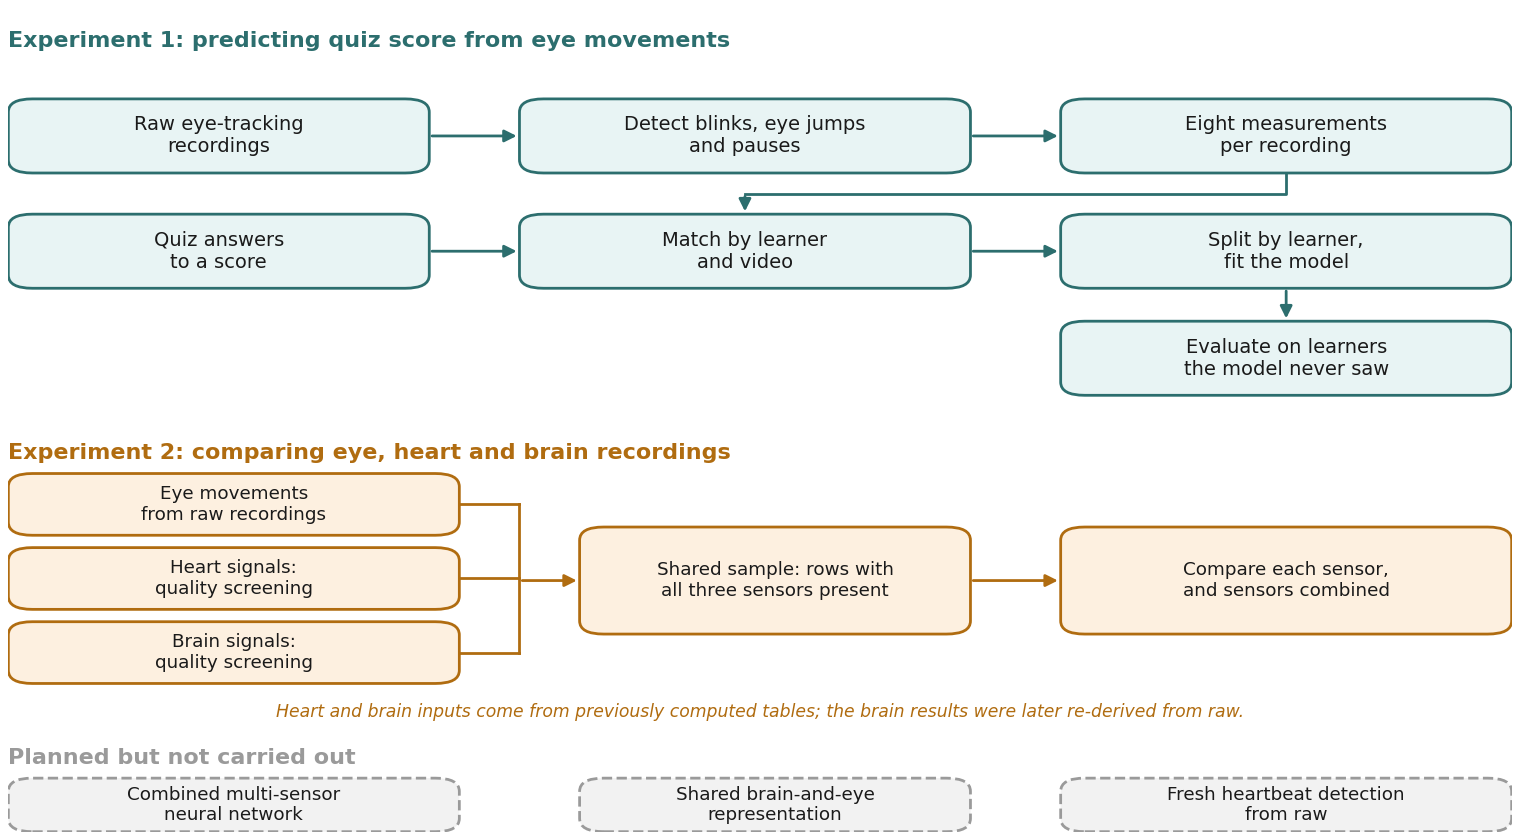
\includegraphics[width=\textwidth,height=0.74\textheight,keepaspectratio]{figures/pipeline_talk.png}

  \sidenote{\reads{Each box is a processing stage. Solid boxes were executed and
  logged; the dashed boxes at the bottom were never run and no results are
  claimed from them. The top band is the completed Experiment 1 eye analysis;
  the middle band is the Experiment 2 multi-sensor comparison. All
  preprocessing is our own, starting from the raw recordings.}}
\end{frame}

% ---------------------------------------------------------------- overview
\begin{frame}{What we ran, in order}
  \small
  \begin{tabular}{@{}p{0.36\textwidth}p{0.58\textwidth}@{}}
    \toprule
    \textbf{Stage} & \textbf{What it established} \\
    \midrule
    Validating the eye pipeline
      & Our own processing reproduces the published attentive-versus-distracted
        differences in eye movement \\
    Predicting quiz score from eye data
      & A weak ordering of learners, with wide uncertainty \\
    Auditing our own analysis code
      & Three implementation defects found and disclosed; the analysis was
        rerun correctly \\
    Building a matched multi-sensor sample
      & 125 learner--video rows with eye, heart and brain data all present \\
    Comparing sensors against each other
      & Brain recording ranked above eye, eye above heart; combining sensors
        did not help \\
    Checking the brain result is not eye artefact
      & Four separate checks, including reprocessing the raw brain recordings \\
    Deep learning
      & Two neural-network experiments; neither beat simple hand-designed
        measurements \\
    \bottomrule
  \end{tabular}

  \vspace{0.6em}
  \sidenote{Each stage is a separately logged analysis run. Where an earlier
  result was superseded, the original was kept unchanged rather than edited.}
\end{frame}

% ---------------------------------------------------------------- RQ0 eye
\begin{frame}{Validation: our pipeline reproduces the published effects}
  \framesubtitle{Experiment 1, 27 learners, 263 recordings \runtag{Run R-004}}
  \centering
  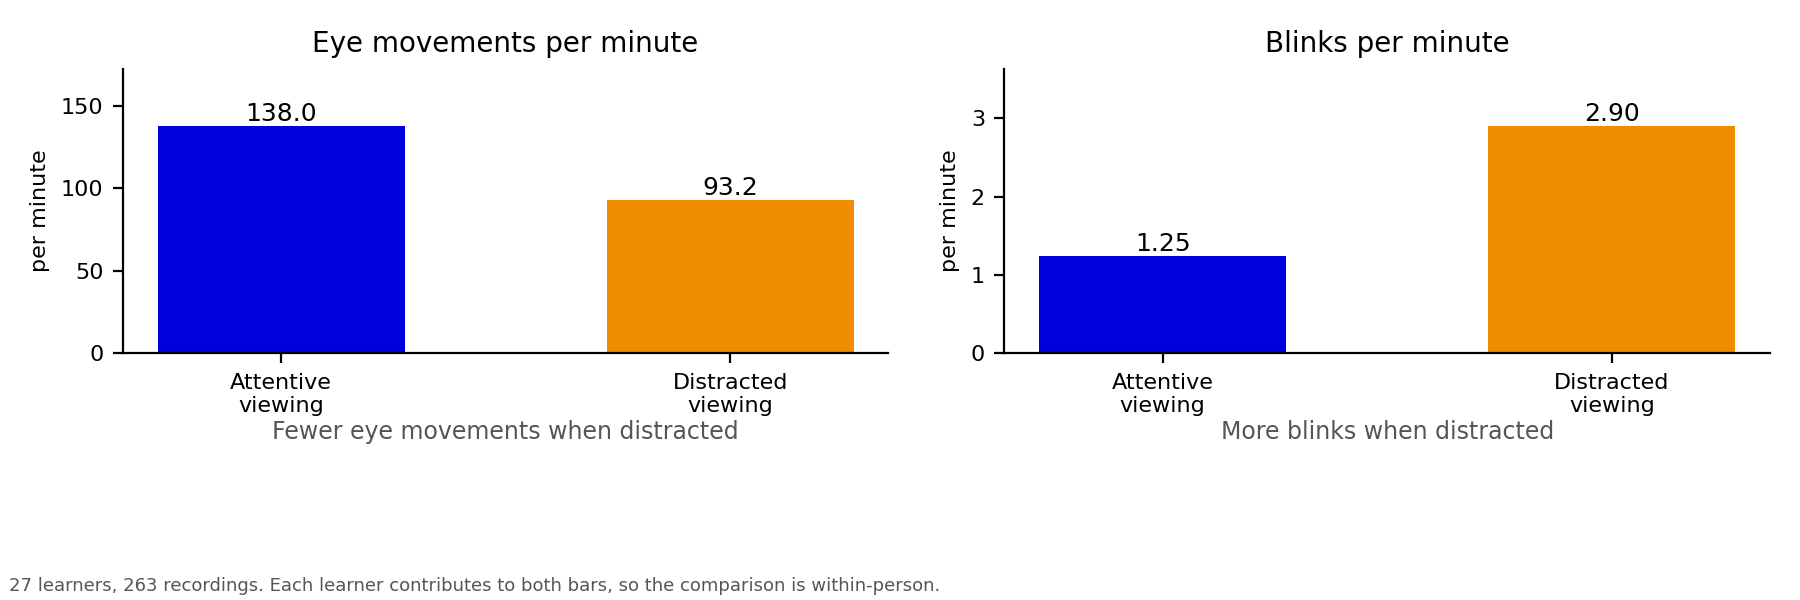
\includegraphics[width=\textwidth,height=0.50\textheight,keepaspectratio]{figures/r004_rates_talk.png}

  \vspace{0.2em}
  {\footnotesize
  Saccades: $t(26) = 6.18$, $p = 1.6\mathrm{e}{-6}$, $d_z = 1.19$ (very large)
  \quad\quad
  Blinks: $t = -3.04$, $p = .005$, $d_z = -0.58$ (medium)}

  \par\vspace{0.2em}
  \raggedright
  \sidenote{\reads{Each pair of bars compares the same learners in the two viewing
  conditions. When distracted, learners made \emph{fewer} eye movements
  (138.0 down to 93.2 per minute) and blinked \emph{more} (1.25 up to 2.90 per
  minute). Both differences match the direction and size reported by the
  dataset's authors, which tells us our processing is working correctly. The
  blink result is the more convincing of the two because blinks are computed
  from pupil data and do not depend on the screen measurement we had to
  infer.}}
\end{frame}

% ---------------------------------------------------------------- audit
\begin{frame}{We audited our own analysis code --- and found three defects}
  \framesubtitle{Disclosed before rerunning, not after seeing the new result}
  \small
  \begin{tabular}{@{}p{0.45\textwidth}p{0.49\textwidth}@{}}
    \toprule
    \textbf{What the first analysis actually did} & \textbf{What the corrected
    analysis does} \\
    \midrule
    Chose the model's strength setting with a shortcut that ignored the
    learner grouping
      & Chooses it inside a properly grouped split, so no learner influences
        their own prediction \\
    The significance test used one data split while the reported result used
    all ten
      & All ten splits refitted for every one of the 1{,}000 permutations \\
    Measured prediction error against the wrong baseline
      & Uses the conventional baseline, and reports the alternative
        separately rather than instead \\
    Corrected for multiple comparisons across one sensor only
      & Leaves the across-sensor correction explicitly unresolved \\
    \bottomrule
  \end{tabular}

  \vspace{0.7em}
  \begin{block}{What this costs us, stated plainly}
    Because the correction was designed \emph{after} seeing the original
    result, it cannot count as a clean confirmatory test, and we do not claim
    it as one. The original analysis and its outputs are preserved unchanged
    rather than overwritten.
  \end{block}
\end{frame}

\begin{frame}{Predicting quiz score from eye movements alone}
  \framesubtitle{Experiment 1, 25 learners, 120 learner--video rows \runtag{Run R-013}}
  \begin{columns}[T]
    \begin{column}{0.44\textwidth}
      \scriptsize
      \begin{tabular}{@{}lr@{}}
        \toprule
        Rank correlation, Spearman $\rho$ & $+0.108$ \\
        95\% confidence interval & $[-0.126, +0.354]$ \\
        Permutation $p$-value & $.032$ \\
        Variance explained, $R^2$ & $-0.031$ \\
        Gain over guessing the mean & $+0.027$ \\
        Mean absolute error & $0.759$ \\
        \bottomrule
      \end{tabular}

      \vspace{0.5em}
      \sidenote{Across the ten repeated splits the correlation ranged from
      $-0.077$ to $+0.279$ --- a single split could easily have shown nothing
      at all.}
    \end{column}
    \begin{column}{0.52\textwidth}
      \begin{block}{Two statistics that disagree --- and both are right}
        \small
        The \textbf{permutation test} asks: could chance alone order learners
        this well? It says probably not ($p = .032$).

        The \textbf{confidence interval} asks: how precisely do we know this
        correlation from only 25 learners? It says barely at all --- the
        interval includes zero.
      \end{block}
      \sidenote{\textbf{What this means:} the eye measurements carry a weak signal
      about who scored better, but not enough to state the effect's size with
      confidence. The negative $R^2$ says the model orders learners slightly
      better than chance while predicting \emph{how much} they scored worse
      than simply guessing the average. We therefore describe this as a weak
      ordering, not a working predictor.}
    \end{column}
  \end{columns}
\end{frame}

% ---------------------------------------------------------------- Exp 2
\begin{frame}{Building a fair multi-sensor comparison}
  \small
  \begin{columns}[T]
    \begin{column}{0.49\textwidth}
      To compare sensors honestly, every sensor must be judged on
      \textbf{exactly the same learners, videos and data splits}. Otherwise a
      sensor could look better simply by being measured on an easier sample.

      \vspace{0.5em}
      \textbf{Eye} --- processed from the raw recordings; 5 recordings
      excluded for poor pupil quality.

      \textbf{Heart} --- we required the heartbeat detector to have found at
      least 80\% of the reference heartbeats: \textbf{140 eligible}, with
      \textbf{15 unevaluable} because processing had failed.

      \textbf{Brain} --- \textbf{139 attentive rows} passed quality control.

      \vspace{0.5em}
      Keeping only rows where all three sensors and a quiz score exist gives
      the shared sample: \textbf{125 learner--video rows, 26 learners,
      5 videos}.
    \end{column}
    \begin{column}{0.47\textwidth}
      \begin{block}{A limitation we state before the results, not after}
        \small
        The heart and brain measurements for this comparison come from
        \textbf{previously computed tables} recovered from our earlier
        processing, not from a fresh run at the time. We verified the code
        that produced them matches our repository, but we cannot certify the
        exact execution.
      \end{block}
      \sidenote{Everything built on those tables is therefore labelled
      exploratory. The brain results were later re-derived from the raw
      recordings, which is reported three slides on. The Experiment 1
      analysis is entirely separate and unaffected.}
    \end{column}
  \end{columns}
\end{frame}

\begin{frame}{Comparing the sensors}
  \framesubtitle{Same 125 rows, same learners, same splits for every sensor \runtag{Run R-017}}
  \centering
  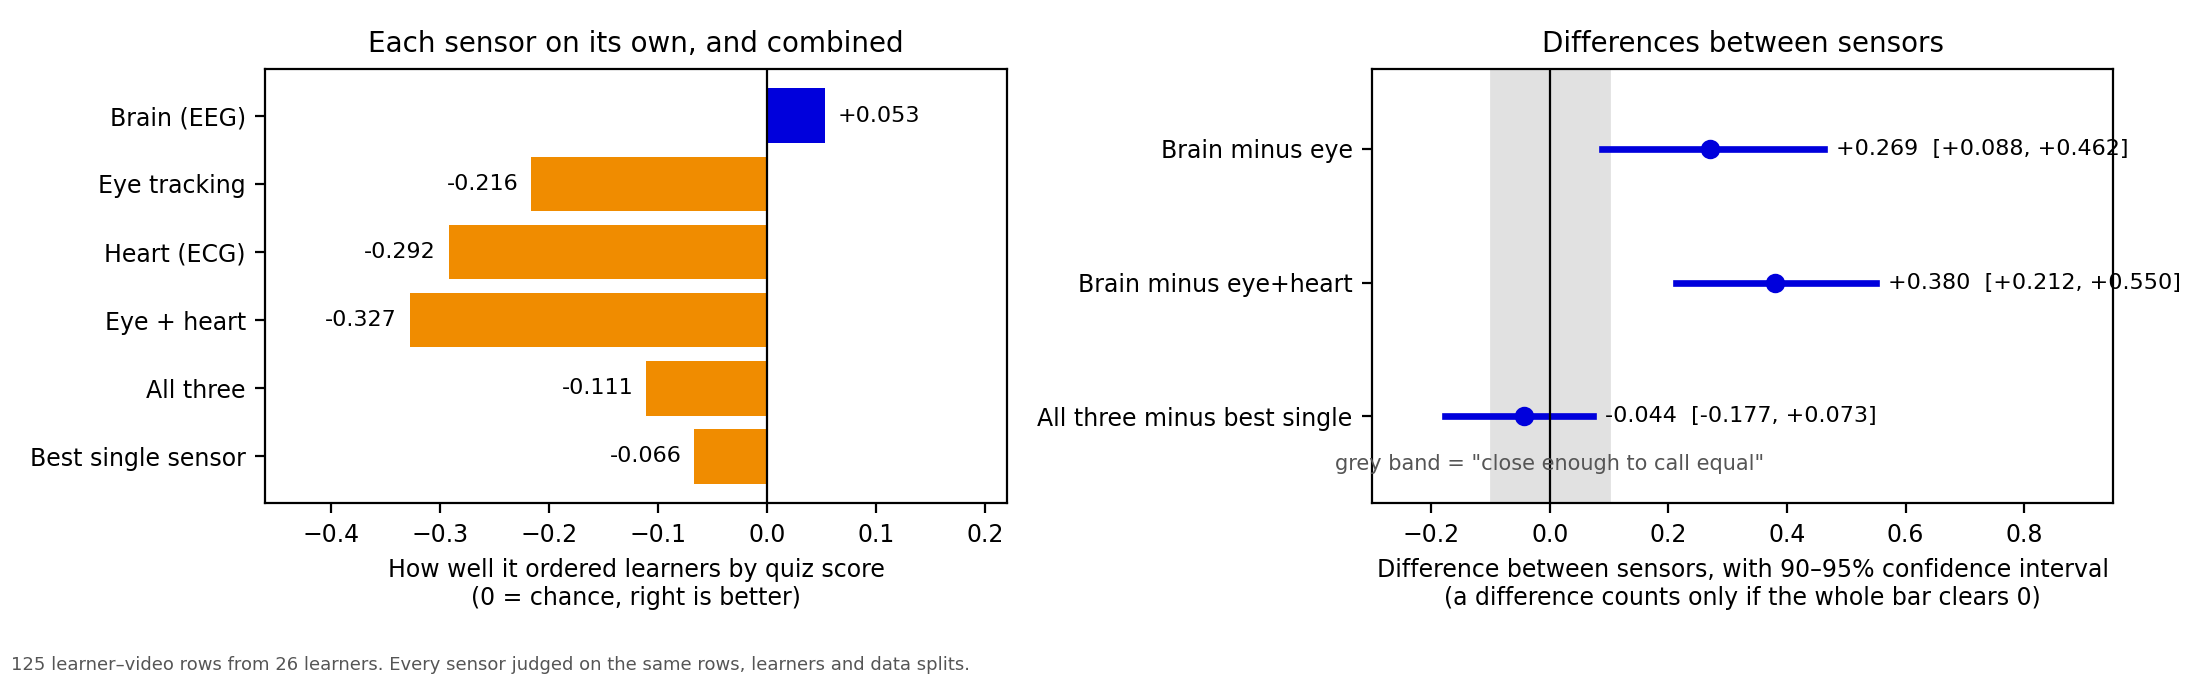
\includegraphics[width=\textwidth]{figures/r017_matched_talk.png}

  \vspace{-0.2em}
  \sidenote{\reads{\emph{Left:} how well each sensor predicted quiz score, as a
  rank correlation. Zero is chance; bars to the left of zero ordered learners
  backwards. \emph{Right:} differences between sensors, with the horizontal
  line showing the 95\% confidence interval. The grey band marks the margin
  within which two sensors would be considered equivalent. A difference is
  established only if its whole interval sits clear of zero.}}
\end{frame}

\begin{frame}{What the sensor comparison does and does not show}
  \begin{columns}[T]
    \begin{column}{0.52\textwidth}
      \textbf{What we can say:}
      \begin{itemize}\small
        \item Brain recording ordered learners better than eye tracking by
          $+.269$, and better than eye and heart combined by $+.380$. Both
          intervals sit clear of zero.
        \item Neither interval fits inside the pre-set equivalence margin, so
          \textbf{we did not show that the cheaper sensors match EEG}.
        \item The eye interval overlaps that margin, so neither did we show
          they are meaningfully \emph{worse}.
        \item Combining all sensors scored $-.044$ against the best single
          sensor, 95\% interval $[-.177, +.073]$ ---
          \textbf{no benefit from combining}.
      \end{itemize}
    \end{column}
    \begin{column}{0.44\textwidth}
      \begin{block}{Four reasons to hold this loosely}
        \small
        \begin{enumerate}
          \item Brain recording itself scored only $+.053$ --- barely above
            chance. A comparison between a weak predictor and weaker ones is
            not a strong claim about EEG.
          \item The intervals resample learners but do not refit the models.
          \item No permutation test was run for this comparison.
          \item The heart and brain inputs come from recovered tables.
        \end{enumerate}
      \end{block}
    \end{column}
  \end{columns}
\end{frame}

% ---------------------------------------------------------------- EEG arc
\begin{frame}{A brain-activity difference between the two conditions}
  \framesubtitle{Experiment 2, 291 recordings, 30 learners \runtag{Run R-018}}
  \begin{columns}[T]
    \begin{column}{0.52\textwidth}
      \scriptsize
      \begin{tabular}{@{}lrr@{}}
        \toprule
        distracted minus attentive & $d_z$ & corrected $p$ \\
        \midrule
        alpha power, rear of head  & $+0.80$ & $.0009$ \\
        alpha power, whole scalp   & $+0.65$ & $.0061$ \\
        alpha share, whole scalp   & $+0.11$ & $1.00$ \\
        alpha share, rear of head  & $-0.00$ & $1.00$ \\
        alpha vs neighbours, whole scalp & $+0.00$ & $1.00$ \\
        alpha vs neighbours, rear of head & $+0.41$ & $.13$ \\
        \midrule
        \textit{delta power, rear of head} & $+0.71$ & --- \\
        \textit{delta power, whole scalp}  & $+0.60$ & --- \\
        \bottomrule
      \end{tabular}

      \vspace{0.4em}
      \sidenote{\reads{Alpha and delta are frequency bands of brain activity.
      Published work reports \emph{alpha specifically} rising when attention
      drops, so our test is whether the rise is confined to alpha.}}
    \end{column}
    \begin{column}{0.44\textwidth}
      \begin{block}{Why we do not claim a replication}
        \small
        Alpha shows the largest effect of any band --- but the rise is
        \textbf{not confined to alpha}. Delta, theta and beta move too, and
        delta shifts furthest of all ($+.143$ against alpha's $+.058$).

        \vspace{0.3em}
        The test designed to isolate alpha --- comparing it against its
        neighbouring frequencies --- gives $d_z = +0.41$ but does not survive
        correction for multiple comparisons ($p = .13$).
      \end{block}
      \sidenote{So brain activity does differ between conditions, but we cannot
      attribute the difference to the alpha band specifically. The next three
      slides ask whether it is a real brain signal at all.}
    \end{column}
  \end{columns}
\end{frame}

\begin{frame}{Is it really brain activity, or just the eyes?}
  \framesubtitle{Test 1 of 3: count blinks in both conditions \runtag{Run R-019}}
  \begin{columns}[T]
    \begin{column}{0.50\textwidth}
      \scriptsize
      \begin{tabular}{@{}lrrr@{}}
        \toprule
        events per minute & attent. & distr. & $d_z$ \\
        \midrule
        \textbf{blinks}   & \textbf{0.00} & \textbf{0.00} & \alert{---} \\
        saccades  & 148.1 & 106.4 & $-1.17$ \\
        fixations & 128.9 &  84.1 & $-1.77$ \\
        \bottomrule
      \end{tabular}

      \vspace{0.5em}
      \sidenote{Saccade and fixation rates reproduce the Experiment 1
      validation, here with condition labels stated in the data files rather
      than inferred. Mean fixation duration is omitted: a few recordings give
      implausible values.}
    \end{column}
    \begin{column}{0.46\textwidth}
      \begin{block}{Blinks were the test --- and there are none to count}
        \small
        Blinking produces large electrical artefacts that can masquerade as
        brain activity, and blinks increase when attention drops. So we
        reprocessed both conditions to count them. \textbf{The blink rate is
        exactly zero in all 302 recordings.}

        \vspace{0.3em}
        This is not a software fault. Of 9.5 million pupil samples only six
        files contain any gap, and five of those are empty throughout.
        \textbf{The published data has already been smoothed}, erasing the
        gaps that mark a blink.
      \end{block}
      \sidenote{A clue: saccades are \emph{fewer} when distracted, so eye
      artefact would be \emph{lower} where brain power is \emph{higher} ---
      the wrong direction to explain it.}
    \end{column}
  \end{columns}
\end{frame}

\begin{frame}{Where on the scalp does the difference appear?}
  \framesubtitle{Test 2 of 3: eye artefact appears at the front of the head \runtag{Run R-020}}
  \begin{columns}[T]
    \begin{column}{0.47\textwidth}
      \scriptsize
      delta power, distracted minus attentive:

      \vspace{0.2em}
      \begin{tabular}{@{}lrr@{}}
        \toprule
        scalp region & $d_z$ & corrected $p$ \\
        \midrule
        rear of head  & $+1.19$ & 4.2e\text{-}06 \\
        front of head & $+1.08$ & 1.3e\text{-}05 \\
        upper rear    & $+1.01$ & 2.5e\text{-}05 \\
        middle        & $+0.70$ & 9.4e\text{-}04 \\
        \midrule
        \textbf{front minus rear}  & $\mathbf{-0.19}$ & $p = .33$ \\
        \bottomrule
      \end{tabular}

      \vspace{0.5em}
      \sidenote{The front-minus-rear difference was fixed as the decisive test
      \emph{before} the run: $-0.0069$, 95\% interval $[-0.0206, +0.0061]$,
      with 42.9\% of learners positive.}
    \end{column}
    \begin{column}{0.49\textwidth}
      \begin{block}{Eye artefact is strongest at the front. This is not.}
        \small
        Blinks and eye movements project most strongly onto electrodes at the
        \textbf{front} of the head, so an eye-driven effect should be much
        larger there. It is not: the front-versus-rear difference is
        indistinguishable from zero, and if anything the effect is
        \emph{largest at the back}.

        \vspace{0.3em}
        \textbf{Evidence against an eye-artefact explanation.}
      \end{block}
      \sidenote{This argues from the pattern rather than correcting anything,
      so it weakens the eye explanation without ruling it out. The next slide
      removes the eye contribution directly.}
    \end{column}
  \end{columns}
\end{frame}

\begin{frame}{Removing the eye contribution directly}
  \framesubtitle{Test 3 of 3: reprocessed from the raw brain recordings \runtag{Run R-021}}
  \begin{columns}[T]
    \begin{column}{0.47\textwidth}
      \scriptsize
      \begin{tabular}{@{}lrrr@{}}
        \toprule
        delta power $d_z$ & before & \textbf{after} & corr.\ $p$ \\
        \midrule
        rear of head  & $+1.24$ & $\mathbf{+1.26}$ & 1.4e\text{-}06 \\
        front of head & $+1.14$ & $\mathbf{+1.06}$ & 1.7e\text{-}05 \\
        upper rear    & $+0.99$ & $\mathbf{+1.03}$ & 1.8e\text{-}05 \\
        middle        & $+0.63$ & $\mathbf{+0.59}$ & 4.1e\text{-}03 \\
        \bottomrule
      \end{tabular}

      \vspace{0.5em}
      \sidenote{\reads{Each recording was processed twice from the same starting
      point --- once with the eye-movement contribution mathematically
      subtracted using dedicated eye electrodes, once without. The only
      difference between the two columns is that subtraction. 264 of 291
      recordings could be used; the other 27 have no eye-electrode file.}}
    \end{column}
    \begin{column}{0.49\textwidth}
      \begin{block}{The effect survives. It is not an eye artefact.}
        \small
        Every region remains statistically significant after the correction,
        and the effect sizes barely move. The largest change is at the front
        of the head and amounts to $-0.08$; the rear regions move slightly
        \emph{upward}.

        \vspace{0.3em}
        A small reduction at the front and none elsewhere is what a little
        eye contamination \emph{sitting on top of a genuine effect} looks
        like. A purely eye-driven effect would have collapsed.
      \end{block}
      \sidenote{Our only brain result computed from the raw recordings rather
      than saved tables. The correction removes what the eye electrodes can
      explain, not eye activity they miss.}
    \end{column}
  \end{columns}
\end{frame}

% ---------------------------------------------------------------- RQ3
\begin{frame}{Does the sensor ranking depend on how we clean the brain data?}
  \framesubtitle{Same 125 rows and splits; only the brain-cleaning method changed \runtag{Run R-022}}
  \begin{columns}[T]
    \begin{column}{0.46\textwidth}
      \scriptsize
      \begin{tabular}{@{}lrr@{}}
        \toprule
        rank correlation & method A & method B \\
        \midrule
        \textbf{brain (EEG)} & $+.080$ & $+.123$ \\
        eye              & $-.216$ & $-.216$ \\
        heart (ECG)      & $-.292$ & $-.292$ \\
        eye + heart      & $-.327$ & $-.327$ \\
        all sensors      & $-.049$ & $-.098$ \\
        best single sensor & $+.025$ & $+.051$ \\
        \bottomrule
      \end{tabular}

      \vspace{0.4em}
      \sidenote{Method A subtracts the eye contribution using eye electrodes.
      Method B separates the recording into independent sources and removes
      the eye-related ones. Eye and heart rows are identical to four decimal
      places --- the check that nothing but the brain data changed.}
    \end{column}
    \begin{column}{0.50\textwidth}
      \begin{block}{The ranking is stable: brain $>$ eye $>$ heart}
        \small
        The ordering is the same under both cleaning methods, and the
        brain-versus-eye advantage sits clear of zero either way. Combining
        sensors still never beats the best single sensor --- under method B
        it is measurably \emph{worse}: $-.149$, 95\% interval
        $[-.291, -.007]$.
      \end{block}
      \sidenote{\textbf{But a stable ordering among weak predictors is a modest
      claim.} Brain recording itself only reaches $+.08$ to $+.12$. The
      second method failed to converge on 19 of the 125 recordings, so that
      column should be read as indicative. This was tested on the exploratory
      Experiment 2 sample, the only place a sensor ranking exists.}
    \end{column}
  \end{columns}
\end{frame}

% ---------------------------------------------------------------- DL
\begin{frame}{Deep learning, part 1: telling the conditions apart}
  \framesubtitle{A neural network reading raw eye signals, tested on unseen learners \runtag{Run R-023}}
  \begin{columns}[T]
    \begin{column}{0.46\textwidth}
      \scriptsize
      \begin{tabular}{@{}lr@{}}
        \toprule
        balanced accuracy per recording & \\
        \midrule
        neural network, 3 runs averaged & \textbf{0.797} \\
        \quad individual runs           & .787 .794 .773 \\
        eight hand-designed measures    & \textbf{0.764} \\
        \midrule
        difference             & $+0.034$ \\
        \bottomrule
      \end{tabular}

      \vspace{0.5em}
      \sidenote{\reads{Balanced accuracy averages accuracy over both
      conditions; 0.5 is chance, 1.0 perfect. 297 recordings, 31 learners,
      36{,}172 four-second windows. The comparison method was fixed
      \emph{before} training, so it could not be chosen to flatter the
      result.}}
    \end{column}
    \begin{column}{0.50\textwidth}
      \begin{block}{It works, but it adds nothing}
        \small
        The network correctly identifies which condition a learner was in
        about 80\% of the time, for learners it has never seen. But its
        $+0.034$ advantage over eight hand-designed numbers is barely larger
        than the \textbf{0.021 variation between its own training runs}, and
        we computed no confidence interval for it. \textbf{We do not claim the
        network is better.}
      \end{block}
      \sidenote{This task is easy by design: eye-movement rate alone nearly
      separates the conditions, so high accuracy shows the pipeline works, not
      that the architecture is good. Identifying \emph{which condition}
      someone was in is also far simpler than predicting \emph{what they
      learned}.}
    \end{column}
  \end{columns}
\end{frame}

\begin{frame}{Deep learning, part 2: predicting what was learned}
  \framesubtitle{Network features versus hand-designed ones, same 125 rows and splits \runtag{Run R-024}}
  \begin{columns}[T]
    \begin{column}{0.46\textwidth}
      \scriptsize
      \begin{tabular}{@{}lr@{}}
        \toprule
        rank correlation with quiz score & \\
        \midrule
        64 network-derived features & $\mathbf{-.077}$ \\
        8 hand-designed measures    & $\mathbf{-.050}$ \\
        \midrule
        difference             & $-.026$ \\
        \quad 95\% interval    & $[-.206, +.158]$ \\
        \bottomrule
      \end{tabular}

      \vspace{0.3em}
      {\scriptsize Individual network runs: $-.102$, $+.009$, $-.048$.}

      \vspace{0.5em}
      \sidenote{The network was retrained from scratch \emph{inside every
      split}, on training learners only. Trained once on everyone, it would
      have shaped its features around the test learners.}
    \end{column}
    \begin{column}{0.50\textwidth}
      \begin{block}{Learned features give no advantage}
        \small
        The network-derived features score slightly \emph{worse}, the
        difference is indistinguishable from zero, and both correlations are
        negative --- neither approach orders learners better than chance on
        this sample. \textbf{On this question, at this sample size, deep
        learning does not help.}
      \end{block}
      \sidenote{Two caveats. One data split rather than ten, so the individual
      values are unstable --- read the \emph{difference}, not the levels. And
      64 features on roughly 100 training rows is unstable in itself, so the
      network is handicapped by having too many features.}
    \end{column}
  \end{columns}
\end{frame}

% ---------------------------------------------------------------- limits
\begin{frame}{Limitations}
  \small
  \begin{itemize}
    \item \textbf{Two inferred assumptions underpin every eye result.} Which
      session was the attentive one, and the screen resolution used to convert
      gaze into degrees. If either is wrong, the eye numbers shift.
    \item \textbf{Only 25--26 learners.} Confidence intervals are necessarily
      wide, and a single unlucky data split could show nothing at all --- which
      is exactly why we repeated every split ten times.
    \item \textbf{No model predicts quiz scores usefully.} Every model orders
      learners at best weakly, and none predicts the actual score better than
      simply guessing the average.
    \item \textbf{One video is too easy} --- 38.7\% of learners scored 90\% or
      above on it, which compresses the very differences we are trying to
      predict.
    \item \textbf{Most heart and brain measurements come from recovered
      tables}, not from a fresh run at the time. The brain results were later
      re-derived from raw recordings; the heart results were not.
    \item \textbf{The correction for testing several sensors at once is
      unresolved}, so every $p$-value here is uncorrected across sensors and
      is presented as such.
  \end{itemize}
\end{frame}

\begin{frame}{What we did not do}
  \begin{block}{Stated plainly, because the project plan promised it}
    \begin{itemize}\small
      \item \textbf{The planned deep-learning track was only partly
        attempted.} We did not build encoders that learn a shared
        representation across brain and eye signals, and we did not build a
        combined multi-sensor network. On a sample of 26 learners these would
        produce numbers we could not interpret or defend, so we chose not to
        run them and recorded that choice in advance.
      \item \textbf{The robustness check was answered on the exploratory
        sample only.} The version planned for the main analysis needs heart
        and brain processing for Experiment 1 that was never completed.
      \item \textbf{The heartbeat detector was never rerun} on the Experiment
        2 raw recordings; we audited the previously saved output instead.
    \end{itemize}
  \end{block}

  \vspace{0.4em}
  \sidenote{We report these as scope decisions rather than omissions, and each
  was logged before the corresponding work was skipped.}
\end{frame}

\begin{frame}{Conclusion}
  \begin{block}{Answering the question we asked}
    On a matched sample with all three sensors present, \textbf{we could not
    show that eye tracking or heart activity matches brain recording} for
    predicting learning, and \textbf{combining sensors gave no benefit} over
    the best single one. But brain recording itself predicted only weakly
    ($\rho = +.053$), so this is evidence about \emph{our} pipeline on
    \emph{this} sample --- not a general verdict on cheap sensors.
  \end{block}

  \vspace{0.3em}
  \begin{itemize}\small
    \item Our processing, built from the raw recordings, reproduces the
      published attention effects in both eye movement and brain activity.
    \item Eye measurements from a single learner carry a weak signal about
      quiz performance for unseen learners, with an interval spanning zero.
    \item The brain-activity difference between conditions is genuine, not an
      eye artefact --- confirmed by reprocessing the raw recordings.
    \item Neither neural network beat simple hand-designed measurements.
    \item We audited our own code, found three defects, and disclosed them
      before reporting the corrected analysis.
  \end{itemize}
\end{frame}

% ---------------------------------------------------------------- refs
\begin{frame}{References}
  \scriptsize
  \begin{enumerate}
    \item J.\ Madsen, N.\ Kuppa and L.\ C.\ Parra, ``The Brain, Body, and
      Behavior Dataset (BBBD): Multimodal Recordings during Educational
      Videos,'' \emph{Scientific Data}, vol.\ 13, art.\ 920, 2026.
    \item S.\ S.\ Cohen et al., ``Neural engagement with online educational
      videos predicts learning performance for individual students,''
      \emph{Neurobiology of Learning and Memory}, vol.\ 155, pp.\ 60--64, 2018.
    \item J.\ Madsen, S.\ U.\ Júlio, P.\ J.\ Gucik, R.\ Steinberg and
      L.\ C.\ Parra, ``Synchronized eye movements predict test scores in
      online video education,'' \emph{PNAS}, vol.\ 118, no.\ 5, e2016980118,
      2021.
    \item J.\ Madsen and L.\ C.\ Parra, ``Cognitive processing of a common
      stimulus synchronizes brains, hearts, and eyes,'' \emph{PNAS Nexus},
      vol.\ 1, no.\ 1, pgac020, 2022.
    \item V.\ J.\ Lawhern et al., ``EEGNet: A compact convolutional neural
      network for EEG-based brain--computer interfaces,'' \emph{Journal of
      Neural Engineering}, vol.\ 15, no.\ 5, 056013, 2018.
    \item G.\ Varoquaux, ``Cross-validation failure: Small sample sizes lead
      to large error bars,'' \emph{NeuroImage}, vol.\ 180, pp.\ 68--77, 2018.
    \item D.\ Makowski et al., ``NeuroKit2: A Python toolbox for
      neurophysiological signal processing,'' \emph{Behavior Research
      Methods}, vol.\ 53, pp.\ 1689--1696, 2021.
    \item A.\ Gramfort et al., ``MEG and EEG data analysis with MNE-Python,''
      \emph{Frontiers in Neuroscience}, vol.\ 7, art.\ 267, 2013.
    \item J.\ Madsen, N.\ Kuppa and L.\ Parra, BBBD, Zenodo dataset record
      19241964.
    \item F.\ Pedregosa et al., ``Scikit-learn: Machine Learning in Python,''
      \emph{JMLR}, vol.\ 12, pp.\ 2825--2830, 2011.
  \end{enumerate}
\end{frame}

\setoutrotext{Thank you}
\makeoutro

\end{document}
